To leverage accelerator and distributed scheduling using the serverless architecture, we have developed STOIC, a framework for executing machine learning applications in hybrid cloud consisting of edge devices and public data centers. The STOIC streamlines the end-to-end process of packaging, transferring, scheduling, executing and retrieving result for machine learning application. Figure~\ref{fig:STOIC} shows the architecture of STOIC, which is composed by three principle pillars: Edge cloud, Mayhem cloud and Nautilus cloud.

\begin{figure}[t] \centering 
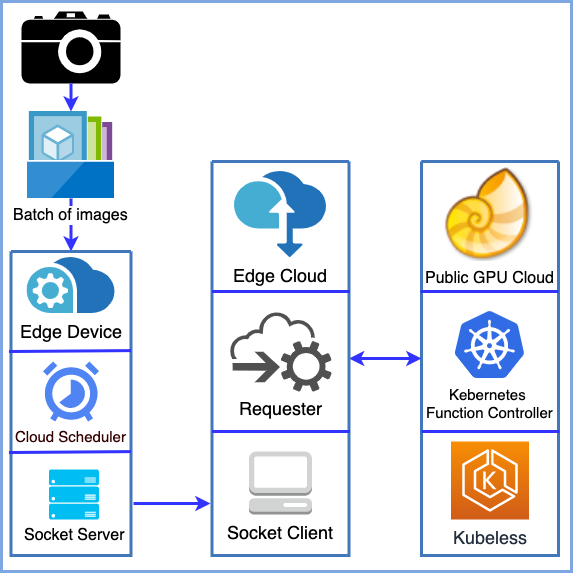
\includegraphics[scale=0.4]{STOIC}
\caption{The architecture of STOIC
\label{fig:STOIC}}
\end{figure}

\subsection{Edge Cloud}
 The edge cloud is a collection of edge devices, including multiple motion-detecting camera traps and local server, deployed in open field and research facility at Sedgwick Natural Reserve~\cite{ref:sedgwick}. Across the field, especially at the water pond, those camera traps are scattered to capture images of wildlife and are connected by microwave link networks to the local server in the research facility. When a motion is detected, the camera traps take photos and persist the images to the attached disk volume. Periodically, they transfer the photos to the local server in the facility, where STOIC socket server constantly listens for batch of images and STOIC cloud scheduler assigns the task to different cloud components. 
 
 \subsection{Mayhem Cloud}
 
 The Mayhem cloud is a private cloud built up by a cluster of nine Intel NUCs~\cite{ref:nucs}. It is managed by Eucalyptus cloud system~\cite{ref:euca} that supports Linux virtual machine instance of Ubuntu and CentOS. Running on an instance, the STOIC socket client listens for the request from edge cloud and STOIC requester interacts with Nautilus Cloud to complete the designated task.
 
 \subsection{Nautilus Cloud}
 
 The Nautilus Cloud~\cite{ref:nautilus} is a HyperCluster research platform led by researchers at UC San Diego, National Science Foundation, Department of Energy and various participating universities globally. Being designed for running data and computation intensive applications, Nautilus uses Kubernetes~\cite{ref:k8s} as interface to manage and scale containerized applications and Rook to automate Ceph~\cite{ref:ceph} data services. As of Nov. 2019, 141 computing nodes across the US joined Nautilus Cloud and 422 GPUs are available in the cluster. We consider Nautilus as an ideal public cloud to leverage accelerators in Serverless architecture to serve edge devices. 
 
 \subsection{Implementation}
 
 \subsubsection{Language}
 Considering performance and interface, STOIC is primarily developed in Golang, since the language provides better performance than scripting language like Python, as well as user-friendly interface~\cite{ref:client-go} to Kubernetes. 
 
 \BlankLine
 \subsubsection{Serverless framework}
 To enable Serverless architecture, STOIC employs kubeless~\cite{ref:kubeless} and Docker~\cite{ref:docker} at Nautilus Cloud. As a kubernetes-native serverless framewrok, kubeless uses CRD (Custom Resource Definition)\cite{ref:crd} to dynamically create functions as kubernetes custom resources and launches runtimes on-demand. For specific machine learning tasks that STOIC executes, we use Docker to build up customized runtime image and upload it to Docker Hub~\cite{ref:dockerhub}. Upon a task request is received, the function controller at Nautilus Cloud pulls the latest image from Docker Hub before launching the function. This deployment pipeline makes the runtime flexible and extensible for future modification. 
 
 \BlankLine
 \subsubsection{Customized Tensorflow}
 To better leverage the computational power of CPU in Edge and Nautilus Cloud, we compile a Tensorflow package from source with AVX2, SSE4.2~\cite{ref:avx} and FMA~\cite{ref:fma} instruction set support. We then test the performance of customized Tensorflow package on three common machine learning training tasks: \textbf{(A)} \textit{Iris}~\cite{ref:iris} with 10-fold cross-validation; \textbf{(B)} \textit{MNIST}~\cite{ref:mnist} on 20 Epochs; \textbf{(C)} \textit{InceptionV3}~\cite{ref:v3} on 10 epochs with 1,000 images. These applications are executed 10 times on both Tensorflow packages to ensure the result is reliable. Table~\ref{tab:avx} describes the performance comparison between two packages. Since the instruction set support accelerates the machine learning task on CPU runtime, we install the customized package to both Edge cloud and Nautilus Cloud Docker image to take advantage of the acceleration.
 
 \BlankLine
 \subsubsection{GPU Accessibility}
 To enable GPU access by Serverless function, we build up our runtime image based off NVIDIA Container Toolkit~\cite{ref:nvidia}. It includes NVIDIA runtime library and utilities to allow Serverless function to leverage NVIDIA GPUs. The resultant image is installed CUDA 10.0 and cuDNN 7.0, which are inline with most GPU nodes' version in Nautilus Cloud. 
 
\begin{table}[]
\centering
\scriptsize

\begin{tabular}{|c|c|c|c|} 
\hline
 & \textbf{Mean Std. (sec)} & \textbf{Mean Custom. (sec)} & \textbf{Speed-up \%}\\
\hline
\textbf{Iris} & 53.17 & 41.86 &  21.3\\
\hline
\textbf{MNIST} & 268.81 & 189.80 & 29.4 \\
\hline
\textbf{InceptionV3} & 958.47 & 791.28 & 17.4 \\
\hline
\end{tabular}

\caption{Performance comparison between standard and customized Tensorflow package}
\label{tab:avx}
\end{table}
 
 \BlankLine
 \subsubsection{Runtime definition}
 To effectively schedule the machine learning tasks, we define four runtime scenarios across hybrid cloud: \textbf{(A)} \textit{edge} - A VM instance at edge cloud on spot with AVX2 support; \textbf{(B)} \textit{cpu} - A pod with CPU with AVX2 support; \textbf{(C)} \textit{gpu1} - A pod with 1 GPU; \textbf{(D)} \textit{gpu2} - A pod with 2 GPUs. The last three runtimes are launched and invoked as kubeless functions at Nautilus Cloud. 
 
 For evaluation and canary release purpose, STOIC has a runtime flag implemented that overrides the runtime selection made by scheduler if the flag is set. This feature extensively helps evaluate the performance of STOIC comparing with single-runtime schedulers.
 
 
 \subsection{Execution Time Estimation}
 Depicted in Figure~\ref{fig:STOIC}, socket server in Edge Cloud keeps listening for images transmitted from camera traps. Upon the end of a preset period (currently 1 hour), STOIC predicts the total time of processing the present batch. The total time includes transfer time, runtime deployment time and corresponding processing time, based on 4 different runtime scenarios. 
 
 \subsubsection{Transfer time} It measures the time spent in transmitting compressed batch of images from Edge Cloud to Mayhem Cloud and Nautilus Cloud. It is calculated as ${T_{tran} = V_{bat} / B}$ where $V_{bat}$ represents the volume of batch and $B$ represents bandwidth at the time provided by a bandwidth monitor at Edge Cloud. 
 
 \subsubsection{Runtime deployment time} It measures the time Nautilus uses to deploy requested kubeless function. Since the scarcity of computation, it is obvious that \textit{gpu2} runtime takes longer to deploy than \textit{gpu1} and \textit{cpu} runtimes. We analyze the deployment log and calculate the average deployment time for each Nautilus runtime. In the future work, we plan to build up feedback control loop to dynamically update deployment time. Kindly notice that, for \textit{edge} runtime, the transfer and runtime deployment time zero out since the task is executed locally in the Edge Cloud.
 
 \subsubsection{Processing time} It is the execution time of specific machine learning task. As the primary component for scheduling task across hybrid cloud, we regress it based on prior experiment data by Bayesian Ridge Regression~\cite{ref:brr} due to its robustness to ill-posted problems compared to Ordinary Least Squares~\cite{ref:ols}. Thus, STOIC formulates the regression and predicts the processing time based on the size of current batch. As same as the deployment time, we plan to construct feedback control loop to dynamically update the coefficient and intercept of regression based on the incoming data of processing time in the future work.
 
 
 \subsection{Workflow}
 Based on three time components aforementioned, the execution times of four scenarios are predicted, and the scheduler selects the runtime with least time. If the choice is \textit{edge} runtime, scheduler will simply execute the task locally in the Edge Cloud. It usually happens when the batch of image is relatively small and does not require much computation from public cloud.
 
 However, when the batch size increases, the task is highly likely to be scheduled at three Nautilus runtimes. For these three scenarios, STOIC sends request, including the payload of compressed image batch and runtime information, to Mayhem Cloud via TCP socket. Upon reception of the request, Mayhem Cloud first requests the deployment of corresponding runtime and secondly sends the payload and request to Nautilus Cloud when the kubeless function is deployed. As a design decision, instead of running a serving pod in Nautilus, we decide to run a server in more stable and fault-tolerant Mayhem Cloud as a relay, due to the intermittent downtime on Nautilus nodes and Ceph storage system. This design provides more reliable infrastructure for tasks executing on STOIC.
 
 On the other end, Nautilus Cloud persists the received images to the shared storage in Ceph file system and monitors the progress of deployment of kubeless function. Once the the serverless function is successfully deployed, Nautilus informs the Mayhem Cloud whose requester will trigger the function via HTTP request. When the task completes, the requester retrieves the results, including the runtime metrics, and transmits them back to Edge Cloud, in which the results and metrics are saved. Up to this point, a full cycle of task execution on Serverless architecture has completed.
 
 \subsection{Intelligent Probing}
 In a series of experiment, we found the processing times of the same image batch and kubeless function vary significantly between first one and following ones. This is caused by cold start~\cite{ref:coldstart} problem of Serverless function. Specifically, most machine learning tasks require retrieval of stored model and dataset from shared file system, which might reside in a separate remote node in Nautilus Cloud. Once they are retrieved and cached in the first invocation, the function can simply use them from the local memory and the performance is boosted dramatically. To approach this issue, STOIC intelligently probes the recently deployed function based on the transition of runtime. When the incoming task is scheduled in a different runtime as previous one, STOIC triggers the function with least amount of data to ensure the model and data are cached in memory and then starts the actual task. Otherwise, to avoid redundant probing, STOIC starts the task directly when the designated runtime is the same as the previous batch. 